% !TEX root = ./Vorlesungsmitschrift AGLA 2.tex  
\lecture{Fr 03.07. 10:15}{}
\chapter{Exkurs: Exponentialabbildungen von Matrizen}
\file{Exponentialabbildungen Matrizen}
\begin{motivation*}[mathematisches Pendel]
  \begin{figure}[H]
    \centering
    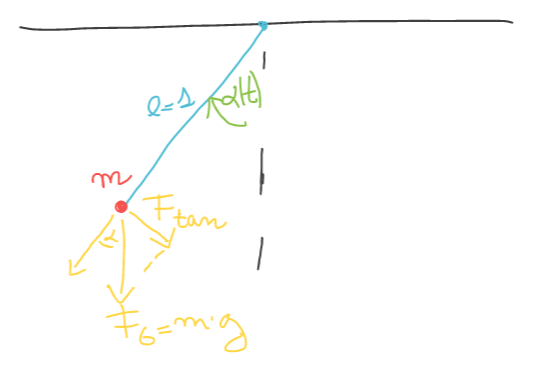
\includegraphics[width=0.5\linewidth]{mathematisches Pendel}
    \label{fig:mathematisches_Pendel}
  \end{figure}
  \begin{equation*}
    F_{\tan}=-mg\Sin-{\alpha(t)}.
  \end{equation*}
  Für kleine Winkel \( \alpha(t) \) ersetze \( \Sin-{\alpha(t)} \) durch \( \alpha(t) \) und erhalte
  \begin{equation*}
    \alpha''(t)=-g \alpha(t).
  \end{equation*}
  Sei \( v(t)=\alpha'(t) \) und erhalte
  \begin{equation*}
    \begin{pNiceMatrix} \alpha'(t) \\ v'(t) \end{pNiceMatrix}=\begin{pNiceMatrix} 0 & 1 \\ -g & 0 \end{pNiceMatrix}\begin{pNiceMatrix} \alpha(t) \\ v(t) \end{pNiceMatrix}.
  \end{equation*}
\end{motivation*}

Allgemeiner sei \( A\in \sqmatrices{n}{\complexs} \), \( y_0\in \complexs^n \). 
\begin{ziel*}
  Finde eine differenzierbare FUnktion \( y\maps \reals\to \complexs^n \) mit \( \odv{y}{}=A\cdot y(t) \) und \( y(0)=y_0 \).
\end{ziel*}
\begin{spezialfall*}[\( n=1 \)]
  Setze \( (t)=y_0 e^{\overbrace{A}^{\mathclap{\subset \reals}}t} \).
\end{spezialfall*}
\begin{idee*}[\( n\geq 1 \)]
  Definiere
  \begin{equation*}
    e^{A t}\definedas \sum_{i=0}^{\infty}\frac{A^i t^i}{\factorial{i}}
  \end{equation*}
  (\( A^0\definedas I_n \)) und setze \( y(t)=e^{A t}y_0 \).
\end{idee*}
\minisec{Formal:}
\begin{equation}
    \odv*{\sum_{i=0}^{\infty}\frac{A^i t^i}{\factorial{i}}}{t}=\sum_{i=0}^{\infty}\frac{\overbrace{A^i}^{AA^{i-1}}\cancel{i}t^{i-1}}{\cancelto{\factorial+{i-1}}{\factorial{i}}}=A \sum_{i=0}^{\infty}\frac{A^i t^i}{\factorial{i}}.
\end{equation}
\begin{frage*}
  Unter welchen Voraussetzungen konvergiert die Reihe
  \begin{equation*}
    \sum_{i=0}^{\infty}\frac{A^i t^i}{\factorial{i}}?
  \end{equation*}
  \tto Wie kann man \( e^{At} \) für \( A\in \sqmatrices{n}{\complexs} \) berechnen? \tto Berechne \( \odv*{e^{At}}{t} \).
\end{frage*}
Sei im Folgenden \( K=\reals \) oder \( K=\complexs \).
\begin{definition*}
  Für \( A\in \sqmatrices{n}{K} \) definiere 
  \begin{equation*}
    e^{A}\definedas \sum_{k=0}^{\infty}\frac{A^k}{\factorial{k}}=I_n+A+\frac{A^2}{2}+\frac{A^3}{6}+\dotsb
  \end{equation*}
  Weiter definiere \( A^0\definedas I_n \) für alle \( A\in \sqmatrices{n}{K} \).
\end{definition*}
\begin{lemma}\label{exponentialabbildung_matrix_absolut_konvergent}
  Sei \( A\in \sqmatrices{n}{K} \). Dann ist die Reihe \( \sum_{k=0}^{\infty}\frac{A^k}{\factorial{k}} \) absolut konvergent (\bzgl einer Norm auf \( \sqmatrices{n}{K} \)).
\end{lemma}
\begin{proof}
  \( \sqmatrices{n}{K}\simeq K^{n^2} \) als \( K \)-Vektorraum, als ind alle Normen auf \( \sqmatrices{n}{K} \) äquivalent. Sei \( \norm{\cdot} \) die Operatornorm auf \( \sqmatrices{n}{K} \), \dh
  \begin{equation*}
    \norm{A}=\sup_{\underline{x}\neq 0}\frac{\norm{Ax}}{\norm{x}}
  \end{equation*}
  mit \( \norm{x} \) und \( \norm{Ax}  \) der euklidischen Norm. Für \( A,B\in \sqmatrices{n}{K} \) ist
  \begin{equation*}
    \norm{AB}\leq \norm{A}\cdot \norm{B}.
  \end{equation*}
  Also gilt
  \begin{align*}
    \norm*{\sum_{k=K_1}^{K_2}\frac{A^k}{\factorial{k}}}&\leq \sum_{k=K_1}^{K_2}\frac{\overbrace{\norm{A^k}}^{\leq \norm{A}^k}}{\factorial{k}}\\
    &\leq \sum_{k=K_1}^{K_2}\frac{\overbrace{\norm{A}}^{\in \reals}{}^k}{\factorial{k}}\goesto 0 \quad (K_1\goesto \infty),
  \end{align*}
  also ist \( \sum_{k=0}^{\infty}\frac{A^k}{\factorial{k}} \) absolut konvergent.
\end{proof}
\begin{korollar}
  Sei \( A\in \sqmatrices{n}{K} \) und \( \varphi\maps \reals\to \sqmatrices{n}{K} \) gegeben durch \( t\mapsto e^{tA} \). Dann ist \( \varphi \) eine differenzierbare Kurve mit
  \begin{equation*}
    \odv*{e^{tA}}{t}=Ae^{tA}.
  \end{equation*}
\end{korollar}
\begin{proof}
  Nach der absoluten Konvergenz gilt
  \begin{align*}
    \odv*{\sum_{k=0}^{\infty}\frac{\p{tA}^k}{\factorial{k}}}{t}&=\odv{\sum_{k=0}^{\infty}\frac{t^k A^k}{\factorial{k}}}{t}\\
    &=\sum_{k=0}^{\infty} k\frac{t^{k-1}A^k}{\factorial{k}}\\
    &=Ae^{tA}.
  \end{align*}
\end{proof}
\subsection*{Weitere Eigenschaften der Exponentialabbildung}
\begin{lemma}
  Seien \( A,B\in \sqmatrices{n}{K} \) und \( T\in \invertiblematrices{n}{K} \). Dann gilt
  \begin{eigenschaftenenumerate}
    \item \label{exponentialabbildung:identitaet} \( e^0=I_n \).
    \item \label{transponiert_konjugiert_funzt_mit_exponentialabbildung} \( e^{\transpose{A}}=\transpose+*{e^A} \) \bzw \( \conjugate{e^A}=e^{\conjugate{A}} \) (für \( A\in \sqmatrices{n}{C} \)).
    \item \label{basiswechsel_funzt_mit_exponentialabbildung} \( e^{TA\inverse{T}}=Te^A\inverse{T} \).
    \item \label{exponentialregel_funzt_mit_exponentialabbildung} \( e^{A+B}=e^{A}\cdot e^{B} \) für \( A,B\in \sqmatrices{n}{K} \) mit \( AB=BA \).
    \item \label{exponentialabbildung:inverses} \( e^A \) ist invertierbar mit \( \inverse+*{e^A}=e^{-A} \) und \( e^{mA}=\p*{e^A}^m \) für \( n\in \wholes \).
  \end{eigenschaftenenumerate}
\end{lemma}
\begin{proof}
  \begin{proofdescription}
    \item[\ref{exponentialabbildung:identitaet}] \begin{equation*}
      e^0\definedas \sum_{k=0}^{\infty}\frac{0^k}{\factorial{k}}=I_n,
    \end{equation*}
    da \( A^0\definedas I_n \) für alle \( A\in \sqmatrices{n}{K} \).
    \item[\ref{transponiert_konjugiert_funzt_mit_exponentialabbildung}]
    \begin{align*}
      e^{\transpose{A}}&=\sum_{k=0}^{\infty}\frac{\p*{\transpose{A}}^k}{\factorial{k}}\\
      &=\sum_{k=0}^{\infty}\frac{\transpose+*{A^k}}{\factorial{k}}\\
      &=\transpose+*{\sum_{k=0}^{\infty}\frac{A^k}{\factorial{k}}}\\
      &=\transpose+*{e^A},
    \end{align*}
    genauso für \( e^{\conjugate{A}} \).
    \item[\ref{basiswechsel_funzt_mit_exponentialabbildung}]
    \begin{align*}
      e^{TA\inverse{T}}&=\sum_{k=0}^{\infty}\frac{\ThisStyle{\overbrace{\SavedStyle(TA\inverse{T})^k}^{\mathclap{TA\ThisStyle{\overbrace{\SavedStyle\inverse{T}T}^{I_n}}A\inverse{T}\dotsm}}}}{\factorial{k}}\\
      &=\sum_{k=0}^{\infty}\frac{T A^k \inverse{T}}{\factorial{k}}\\
      &=Te^A \inverse{T}.
    \end{align*}
    \item[\ref{exponentialregel_funzt_mit_exponentialabbildung}] Sei \( AB=BA \). Betrachte
    \begin{align*}
      e^{A+B}&=\sum_{k=0}^{\infty}\frac{(A+B)^k}{\factorial{k}}\\
      &\explain[big]{AB=BA}{=}\sum_{k=0}^{\infty}\sum_{l=0}^{k}\begin{pNiceMatrix} k \\ l \end{pNiceMatrix}\frac{A^l B^{k-l}}{\factorial{k}}\\
      &=\sum_{k=0}^{\infty}\sum_{l=0}^{k}\frac{A^l B^{k-l}}{\factorial{l}\factorial+{k-l}}\\
      &=\sum_{l=0}^{\infty}\sum_{k=0}^{\infty}\frac{A^l B^{k-l}}{\factorial{l}\factorial+{\braceannotate{l'}{k-l}}}\\
      &=\sum_{l=0}^{\infty}\sum_{l'=0}^{\infty}\frac{A^l}{\factorial{l}}\frac{B^{l'}}{\factorial+{l'}}=e^A \cdot e^B
    \end{align*}
    \item[\ref{exponentialabbildung:inverses}] Für \( m\geq 0 \) folgt
    \begin{equation*}
      e^{mA}=\p*{e^A}^m
    \end{equation*}
    induktiv aus \ref{exponentialregel_funzt_mit_exponentialabbildung}, denn \( (m-1)A \) und \( A \) kommutieren. Weiter ist
    \begin{equation*}
      I_n=e^0=e^{A-A}\explain{\text{\ref{basiswechsel_funzt_mit_exponentialabbildung}}}{=}e^A\cdot e^{-A}
    \end{equation*}
    nach \ref{exponentialregel_funzt_mit_exponentialabbildung} also \( e^{-A}=\inverse+{e^A} \).
  \end{proofdescription}
\end{proof}
\begin{bemerkungen*}
  \begin{itemize}
    \item Insbesondere 
    \begin{equation*}
      e^A\in \invertiblematrices{n}{K}
    \end{equation*}
    für alle \( A\in \sqmatrices{n}{K} \).
    \item Im Allgemeinen ist \( e^{A+B}\neq e^A\cdot e^B \). Betrachte \zb
    \begin{equation*}
      A=\begin{pNiceMatrix} 0 & 1 & 0 \\ 0 & 0 & 0 \\ 0 & 0 & 0 \end{pNiceMatrix},\quad B=\begin{pNiceMatrix} 0 & 0 & 0 \\ 0 & 0 & 1 \\ 0 & 0 & 0 \end{pNiceMatrix},\quad C=\begin{pNiceMatrix} 0 & 0 & 1 \\ 0 & 0 & 0 \\ 0 & 0 & 0 \end{pNiceMatrix}.
    \end{equation*}
    Nachrechnen ergibt
    \begin{equation*}
      e^{A+B}=I_3+A+B+\frac{1}{2}C
    \end{equation*}
    und
    \begin{align*}
      e^A\cdot e^B&=(I_3+A)(I_3+B)\\
      &=I_3+A+B+C.
    \end{align*}
  \end{itemize}
\end{bemerkungen*}
\begin{satz}
  Seien \( A,B\in \sqmatrices{n}{K} \) fest und \( t\in \reals \). Dann gilt für \( \abs{t}\leq 1 \)
  \begin{equation*}
    e^{tA}e^{tB}-e^{t(A+B)}=\frac{t^2}{2}(AB-BA)+O(t^3).
  \end{equation*}
\end{satz}
\begin{proof}
  Aus der Reihenentwicklung erhalten wir
  \begin{align*}
    e^{t(A+B)}&=I_n+t(A+B)+\frac{t^2}{2}(A+B)^2+\braceannotate{=O(t^3)}{\sum_{k=3}^{\infty}\frac{t^k(A+B)^k}{\factorial{k}}}\\
    &=I_n+t(A+B)+\frac{t^2}{2}(A^2+AB+BA+B^2)+O(t^3)
  \end{align*}
  und
  \begin{align*}
    e^{tA}e^{tB}&=\p*{I_n+tA+\frac{t^2}{2}A^2+O(t^3)}\p*{I_n+tB+\frac{t^2}{2}B^2+O(t^3)}\\
    &=I_n+tA+tB+t^2AB+\frac{1}{2}t^2(A^2+B^2)+O(t^3).
  \end{align*}
\end{proof}
\begin{beispiele*}[zur Berechnung der Exponentialabbildung]
  \begin{enumerate}
    \item\label{exponentialabbildung:diagonalmatrix} Sei \( D\in \sqmatrices{n}{K} \) eine Diagonalmatrix mit
    \begin{equation*}
      D=\begin{pNiceMatrix} \lambda_1 &  & 0 \\  & \Ddots &  \\ 0 &  & \lambda_n \end{pNiceMatrix}.
    \end{equation*}
    Dann ist
    \begin{equation*}
      e^D=\begin{pNiceMatrix} e^{\lambda_1} &  & 0 \\  & \Ddots &  \\ 0 &  & e^{\lambda_n} \end{pNiceMatrix}.
    \end{equation*}
    \item\label{exponentialabbildung:abwechselmatrix} Sei \( A=\begin{pNiceMatrix} 0 & \beta \\ -\beta & 0 \end{pNiceMatrix} \) mit \( \beta\in \reals \). Dann ist
    \begin{align*}
      A^2&=\begin{pNiceMatrix} -\beta^2 & 0 \\ 0 & -\beta^2 \end{pNiceMatrix}=-\beta^2\cdot I_2\\
      A^3&=-\beta^2A\\
      A^4&=\beta^4 I_2.
    \end{align*}
  Also
  \begin{align*}
    e^A&=\sum_{k=0}^{\infty}\frac{A^k}{\factorial{k}}\\
    &=\sum_{k=0}^{\infty}\frac{A^{2k+1}}{\factorial+{2k+1}}+\sum_{k=0}^{\infty}\frac{A^{2k}}{\factorial+{2k}}\\
    &=\sum_{k=0}^{\infty}\frac{1}{\factorial+{2k+1}}(-1)^k \beta^{2k}A+\sum_{k=0}^{\infty}\frac{1}{\factorial+{2k}}(-1)^k \beta^{2k}I_2,
  \end{align*}
  also
  \begin{align*}
    e^A&=\Sin+{\beta}\begin{pNiceMatrix} 0 & 1 \\ -1 & 0 \end{pNiceMatrix}+\Cos+{\beta}I_2\\
    &=\begin{pNiceMatrix} \Cos+{\beta} & -\Sin+{\beta} \\ \Sin+{\beta} & \Cos+{\beta} \end{pNiceMatrix}.
  \end{align*}
  \item\label{verschobene_einheitsmatrix} Sei \( A\in \sqmatrices{n}{\complexs} \) gegeben durch 
  \begin{equation*}
    A=\begin{pNiceMatrix} 0 & 1 & 0 & \Cdots & 0 \\   \Vdots & \Ddots & \Ddots & \Ddots & \Vdots \\  &  & & & 0 \\ & & & & 1 \\ 0 & \Cdots & &  & 0 \end{pNiceMatrix}.
  \end{equation*}
  Dann ist
  \begin{equation*}
    A^2=\begin{pNiceMatrix} 0 &  0 & 1 & 0 & \Cdots & 0 \\   \Vdots & \Ddots & \Ddots & \Ddots & \Ddots & \Vdots \\  & & & & & 0 \\ & && & & 1 \\  & & & &  & 0 \\ 0&\Cdots & & && 0\end{pNiceMatrix},\quad A^n=0
  \end{equation*}
  und
  \begin{equation*}
    e^{tA}=\begin{pNiceMatrix} 0 & t & \frac{t^2}{2} & \Cdots & \frac{t^{n-1}}{\factorial+{n-1}} \\   \Vdots & \Ddots & \Ddots & \Ddots & \Vdots \\  &  & & & \frac{t^2}{2} \\ & & & & t \\ 0 & \Cdots & &  & 0 \end{pNiceMatrix}.
  \end{equation*}  
  \end{enumerate}
\end{beispiele*}
\begin{frage*}
  Wie kann man für eine allgemeine Matrix \( A\in \sqmatrices{n}{\complexs} \) die Exponentialabbildung \( e^A \) explizit berechnen?
\end{frage*}
\begin{idee*}
  Reduziere nach Konjugation auf die Beispiele \ref{exponentialabbildung:diagonalmatrix} und \ref{verschobene_einheitsmatrix}.
\end{idee*}
\begin{erinnerung*}[Jordansche Normalform]
  Sei \( A\in \sqmatrices{n}{\complexs} \) mit paarweise verschiedenen Eigenwerten \( \lambda_1,\dotsc,\lambda_k \). Dann gibt es eine invertierbare Matrix \( T\in \invertiblematrices{n}{\complexs} \) mit
  \begin{equation*}
    \inverse{T}A T=\begin{pNiceMatrix} \boxed{\lambda_1 I_{r_1}+N_1} &  &  \\  & \Ddots &  \\  &  & \boxed{\lambda_k I_{r_k}+N_k} \end{pNiceMatrix},
  \end{equation*}
  wobei \( r_1+\dotsb+r_k=n \) und
  \begin{equation}
    N_i=\begin{pNiceMatrix} 0 & * & 0 & \Cdots & 0 \\   \Vdots & \Ddots & \Ddots & \Ddots & \Vdots \\  &  & & & 0 \\ & & & & * \\ 0 & \Cdots & &  & 0 \end{pNiceMatrix}
  \end{equation}
  mit \( *\in \Set{0,1} \).
\end{erinnerung*}
\subsection*{Anwendung auf die Berechnung des Exponentialabbildung}
Sei \( A\in \sqmatrices{n}{\complexs} \) und \( T\in \invertiblematrices{n}{\complexs} \) mit \( \inverse{T}AT=D+N \) mit
\begin{align*}
  D&=\begin{pNiceMatrix} \lambda_1 &&&&&&0  \\  & \Ddots    \\  &  & \lambda_1 \\ &&&\Ddots \\
   &&&&\lambda_k \\&&&&&\Ddots \\0 &&&&&&\lambda_k \end{pNiceMatrix}\\
  N&=\begin{pNiceMatrix} 0 & * & 0 & \Cdots & 0 \\   \Vdots & \Ddots & \Ddots & \Ddots & \Vdots \\  &  & & & 0 \\ & & & & * \\ 0 & \Cdots & &  & 0 \end{pNiceMatrix}
\end{align*}
mit \( *\in \set{0,1} \). Dann \( DN=ND \).

Wir erhalten
\begin{align*}
  e^{tA}&=e^{T(t(D+N))\inverse{T}}\\
  &=Te^{t(D+N)}\inverse{T}\\
  &=Te^{tD+tN}\inverse{T}\\
  &=T e^{tD}\cdot e^{tN}\inverse{T}.
\end{align*}
Für \( e^{tD} \) und \( e^{tN} \) verwende die Beispiele \ref{exponentialabbildung:diagonalmatrix} und \ref{verschobene_einheitsmatrix} 

\subsection*{Eine weitere Folgerung aus der Jordanschen Normalform}

\begin{definition*}
  Sei \( A=\p*{a_{ij}}_{1\leq i,j\leq n}\in \sqmatrices{n}{\complexs} \). Setze \( \trace+{A}=\sum_{i=1}^{n}a_{ii} \).
\end{definition*}
\begin{bemerkung*}
  Es gilt
  \begin{equation*}
    \trace+{AB}=\trace+{BA}\quad \forall A,B\in \sqmatrices{n}{\complexs}.
  \end{equation*}
\end{bemerkung*}
\begin{lemma}
  Sei \( A\in \sqmatrices{n}{\complexs} \). Dann ist
  \begin{equation*}
    \determinant-{e^A}=e^{\trace{A}}.
  \end{equation*}
\end{lemma}
\begin{proof}
  Sei \( T\in \invertiblematrices{n}{\complexs} \), sodass \( \inverse{T}AT=D+N \) in Jordanscher Normalform ist. Es ist
  \begin{equation*}
    \trace+{A}=\trace+{T\inverse{T} A}=\trace+{\inverse{T}AT}=\trace+{D+N}
  \end{equation*}
  und 
  \begin{equation*}
    \determinant{e^A}=\determinant{e^{T(D+N)\inverse{T}}}=\determinant+*{Te^{D+N}\inverse{T}}=\determinant{e^{D+N}}.
  \end{equation*}
  Es genügt also das Lemma für \( D+N \) nachzuweisen. Sei
  \begin{equation*}
    D=\begin{pNiceMatrix} \lambda_1 &  & 0 \\  & \Ddots &  \\ 0 &  & \lambda_n \end{pNiceMatrix}, \quad \lambda_i\in \complexs.
  \end{equation*}
  Direkte Rechnung ergibt 
  \begin{equation*}
    \determinant{e^{D+N}}=e^{\lambda_1}\dotsm e^{\lambda_n}=e^{\lambda_1+\dotsb+\lambda_n}=e^{\trace+{D+N}}.
  \end{equation*}
\end{proof}
